\documentclass[acmtog]{acmart}
\usepackage{graphicx}
\usepackage{subfigure}
\usepackage{natbib}

% Title portion
\title{Assignment 5 : Rendering Isosurfaces by Volumetric Techniques} 
\author{Student Name Zhanrui Zhang\quad Student No. 2019533227 \\ Email: zhangzhr2@shanghaitech.edu.cn}

% Document starts
\begin{document}
\maketitle

\vspace*{2 ex}


\section{Introduction}

In this assignment, we are required to inplement a volume renderer to render some isosurfaces. A classifier is defined to display the gradient of specified isosurface, with Phong lighting model applied on the rendered surface.

\section{Implementation Details}

\subsection{Front to Back Volume Rendering}
For each ray, we first test the ray intersection with the bounding box. We can obtain the t\_in and t\_out if the ray intersects with the bounding box. Then we marching the ray by step set in the config file from t\_in to t\_out. We need to keep track of two variables, color $C$ and opacity $\alpha$. For fornt to back volume rendering: 
\[C_{dst} = C_{dst} + (1-\alpha_{dst}) \cdot C_{src}\]
\[\alpha_{dst} = \alpha_{dst} + (1-\alpha_{dst}) \cdot \alpha_{src}\]

For marching ray, we update the color and opacity by above equation. When the opacity reaches 1, we terminate the ray to save time.

\subsection{Classifier: color and transparency of given position}
In out classifier, we need to calculate the color and transparency of given position.

For transparency, we need to return 1 for all position that is not on the isosurface, and return 0 for all position that is on the isosurface. Here we use a gauss function to make results more friendly to numerical computing.
The gauss function is given as:
\[f(t) = \frac{1}{\sigma\sqrt{2\pi}}\exp(-\frac{(t-t0)^2}{2\sigma^2})\]

In my implementation, I calculated 
\(\exp(-\frac{t^2}{2\mathrm{dt}^2})\), if the result is larger than 0.6, then we consider the point is on the isosurface.

If current point of the marching ray is on the isosurface (or very close to the isosurface), then we set current transparency to zero. The base color is given by the x normal. We can apply a color map to map different value of x normal to different color. Then we apply Phong model on the isosurface to calculate the final color. 

The key here is to get the normal of the isosurface, since the implicit expression of the surface, we can easily get the normal by calculate the gradient of the surface and normalize it. Gradient can be calculated directly based on the expression of the surface, and can be directly evaluated for given position.

\subsection{Simultaneously render multiple isosurfaces}
To render multiple isosurfaces simultaneously, we need to add multiple geometry to the scene.
We construct a overall bounding box for all objects. In the rendering process, we calculate the isosurface value for each objects. Once the transparency is below zero, we terminate the ray.

\section{Results}
\begin{figure}[h]
    \centering
    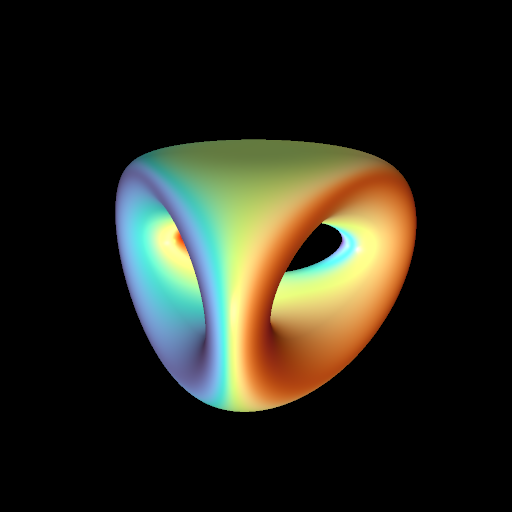
\includegraphics[scale=0.35]{../Coding/images/fw_genus2_x_grad.png}
    \caption{Genus2 x-normal}
\end{figure}

\begin{figure}[h]
    \centering
    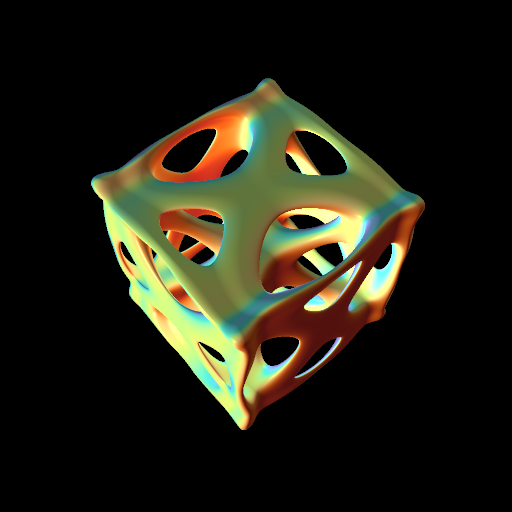
\includegraphics[scale=0.35]{../Coding/images/fw_porous_surf.png}
    \caption{Porous x-normal}
\end{figure}

\begin{figure}[h]
    \centering
    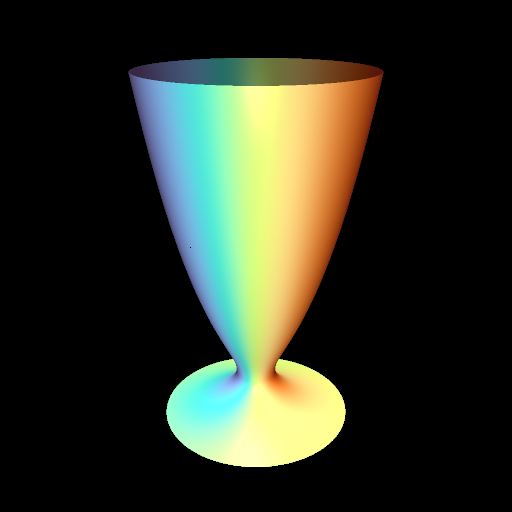
\includegraphics[scale=0.35]{../Coding/images/fw_wineglass.png}
    \caption{Wineglass x-normal}
\end{figure}

\begin{figure}[h]
    \centering
    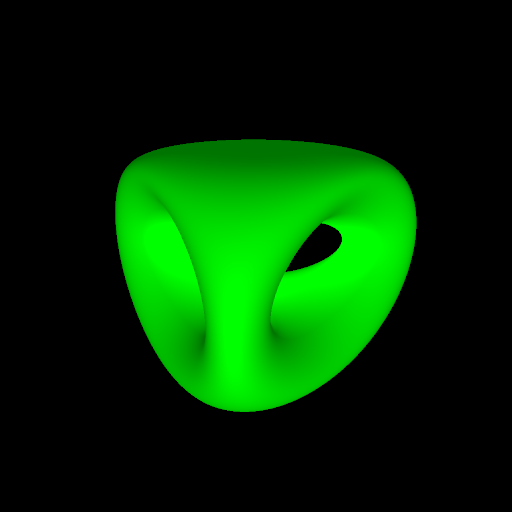
\includegraphics[scale=0.35]{../Coding/images/fw_genus2_pure_color.png}
    \caption{Genus2 pure color}
\end{figure}

\begin{figure}[h]
    \centering
    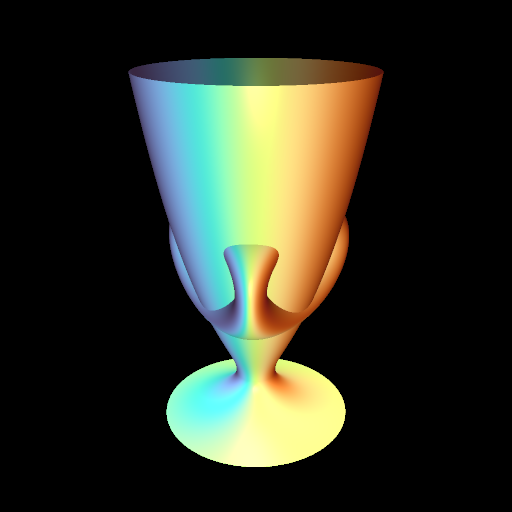
\includegraphics[scale=0.35]{../Coding/images/wineglass_genus2.png}
    \caption{Multiple Objects}
\end{figure}

\end{document}
